\graphicspath{{./Figs/}}

\chapter{Progress} 
The current progress completed is focused on a review of areas of research that are relevant to the main topic of this thesis. An analysis of current MAV optimisation techniques was conducted, and the development of a reasonable MAV baseline model is currently underway. The design and 3D print of a MAV model, which can be tested in different configurations, is also currently in progress. 

\section{Problem Analysis}
\label{sec: ProblemAnalysis}
In order to understand the context of currently completed work, it is essential to understand the main goal of this investigation. The main investigation of this thesis is to analyse the effects of propeller-wing interactions and determine how these affect small MAV aircraft. 

\section{Currently Completed Work}
\label{sec: completedWork}

In order to analyse the propeller wing effects of a MAV in experimental testing, initial investigations of current baseline models were conducted to determine what shapes of aircraft are currently modelled. The aircraft generation code provided by Professor Dries Verstraete has been modified in order to produce a MAV design that has suitable characteristics for use in experimental testing.

A current example of this is, again, the GenMAV model.
\cite{Stewart2007} which does not allow for the addition of a propeller to test for the propeller interaction effects as seen in Figure \ref{fig:genmav2}. An alternative design is suggested based on the NanoTalon as shown in Figure \ref{fig:NanoTalon}. The shape of this design, however, is optimised for manufacturability while still being testable within a wind tunnel, and in doing so, this aircraft loses a typical streamlined fuselage shape. 


\begin{figure}[H]
    \centering
    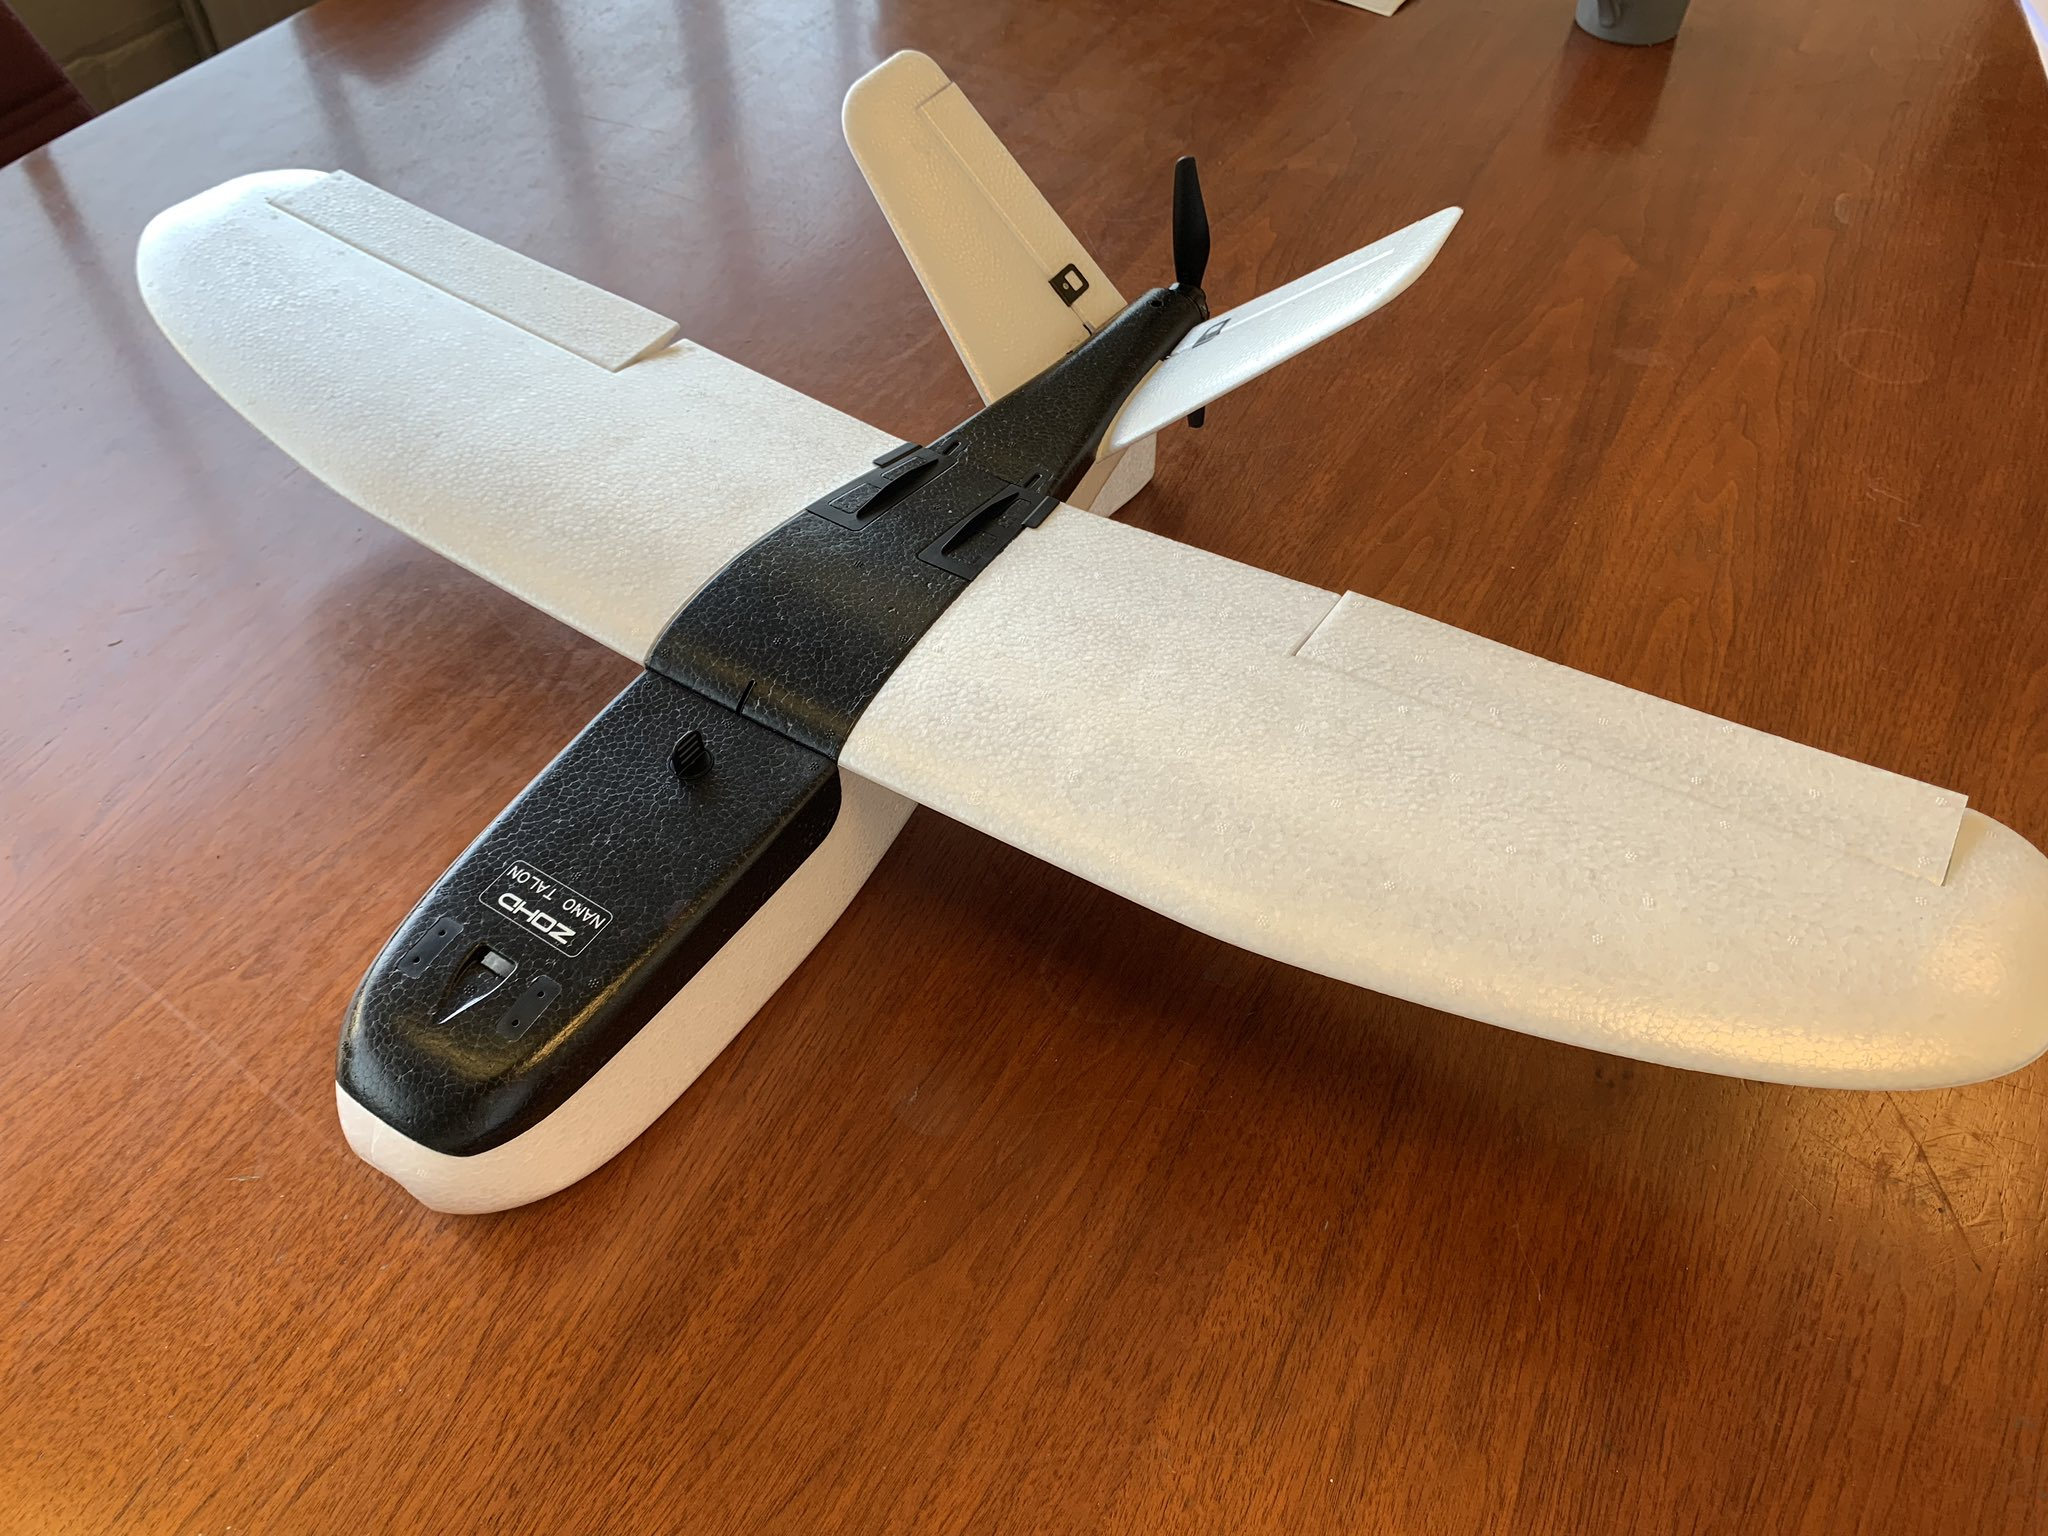
\includegraphics[width=0.7\linewidth]{04_Progress/Figs/DwfPl1HWwAA6nSd.png}
    \caption{NanoTalon Model \cite{NanoTalon2}}
    \label{fig:NanoTalon}
\end{figure}

The main fuselage of the model, which is still being developed, takes into account the importance of interchangeability in order to add and remove a propeller. It also considers that most aircraft will generally have a streamlined body shape, as shown in Figure \ref{fig:model}.
%Add image of the model

\begin{figure}[H]
    \centering
    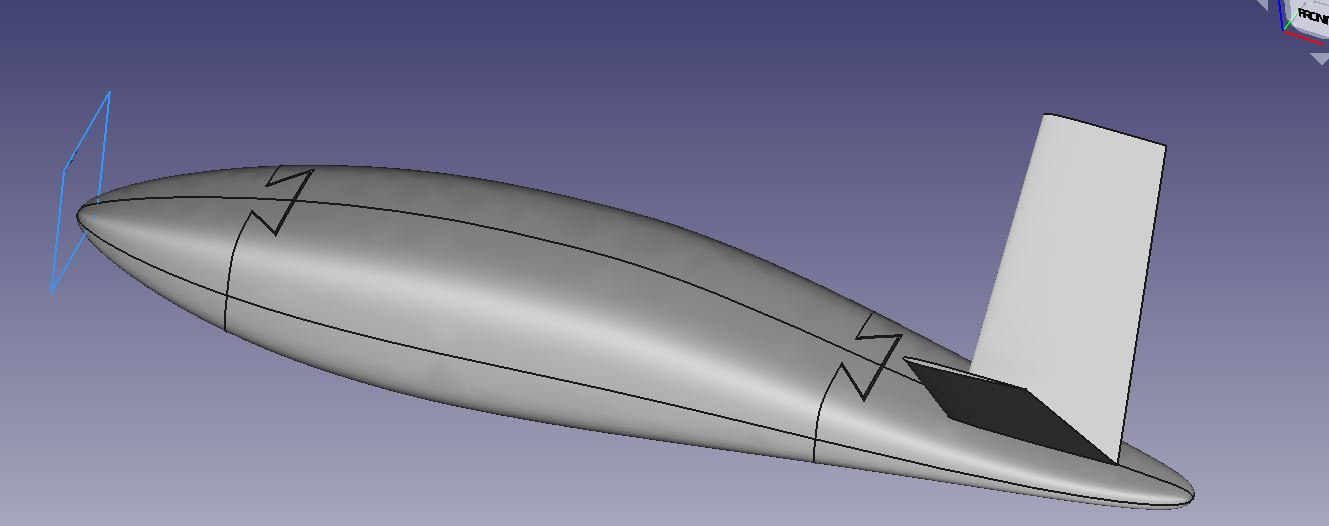
\includegraphics[width=\linewidth]{04_Progress/Figs/model.JPG}
    \caption{Current Model}
    \label{fig:model}
\end{figure}

Due to the complexity of the wing shape and airfoil, the main wing was modelled in VSP software and based on a model of the NanoTalon as shown in Figure \ref{fig:openVSP}. 

\begin{figure}[H]
    \centering
    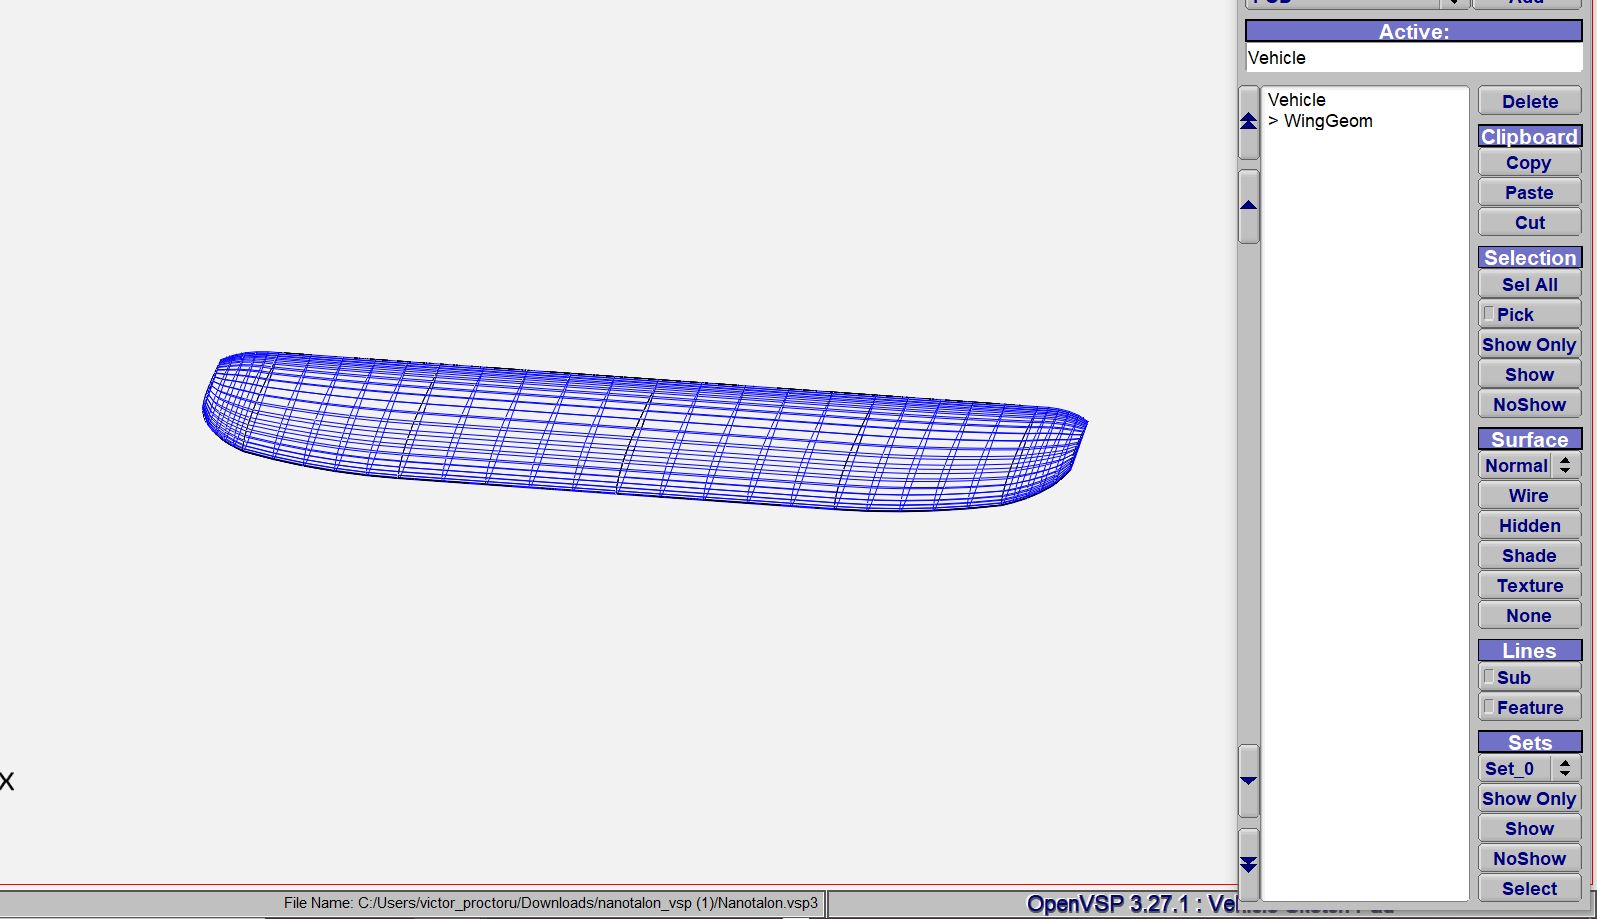
\includegraphics[width=\linewidth]{04_Progress/Figs/openVSp.JPG}
    \caption{Open VSP model of wing design based on NanoTalon \cite{NanoTalon}}
    \label{fig:openVSP}
\end{figure}

This wing design was chosen due to its generic wing shape and simple design. The main geometry of the current model is given in Figure \ref{fig:model}.



The general geometry uses a NACA4412 airfoil with a wingspan of 860 mm and a max chord length of 183 mm. The main fuselage shape was modelled in order to represent a generic streamlined aircraft body shape. The main geometry features were based on the NanoTalon, although modified in order to better allow for a propeller to be attached and tested while operating. The tailpiece is cut before the end in the model shown in Figure \ref{fig:model} due to the thickness being too small to use as a wind tunnel experimental model.

Experimental 3D models have been printed to determine the feasibility of the widths of certain sections, as shown in Figure \ref{fig:3Dmodel}, in order for the model to carry the main propeller and battery. Consideration of the assembly of the main structure must also be considered, and hence these initial prints provide validation into whether the current thicknesses are reasonable or will need to be adjusted. An example of the attachable headpiece is shown in Figure \ref{fig:3Dmodel}, which was testing the feasibility of an interchangeable model. 

\begin{figure}[H]
    \centering
    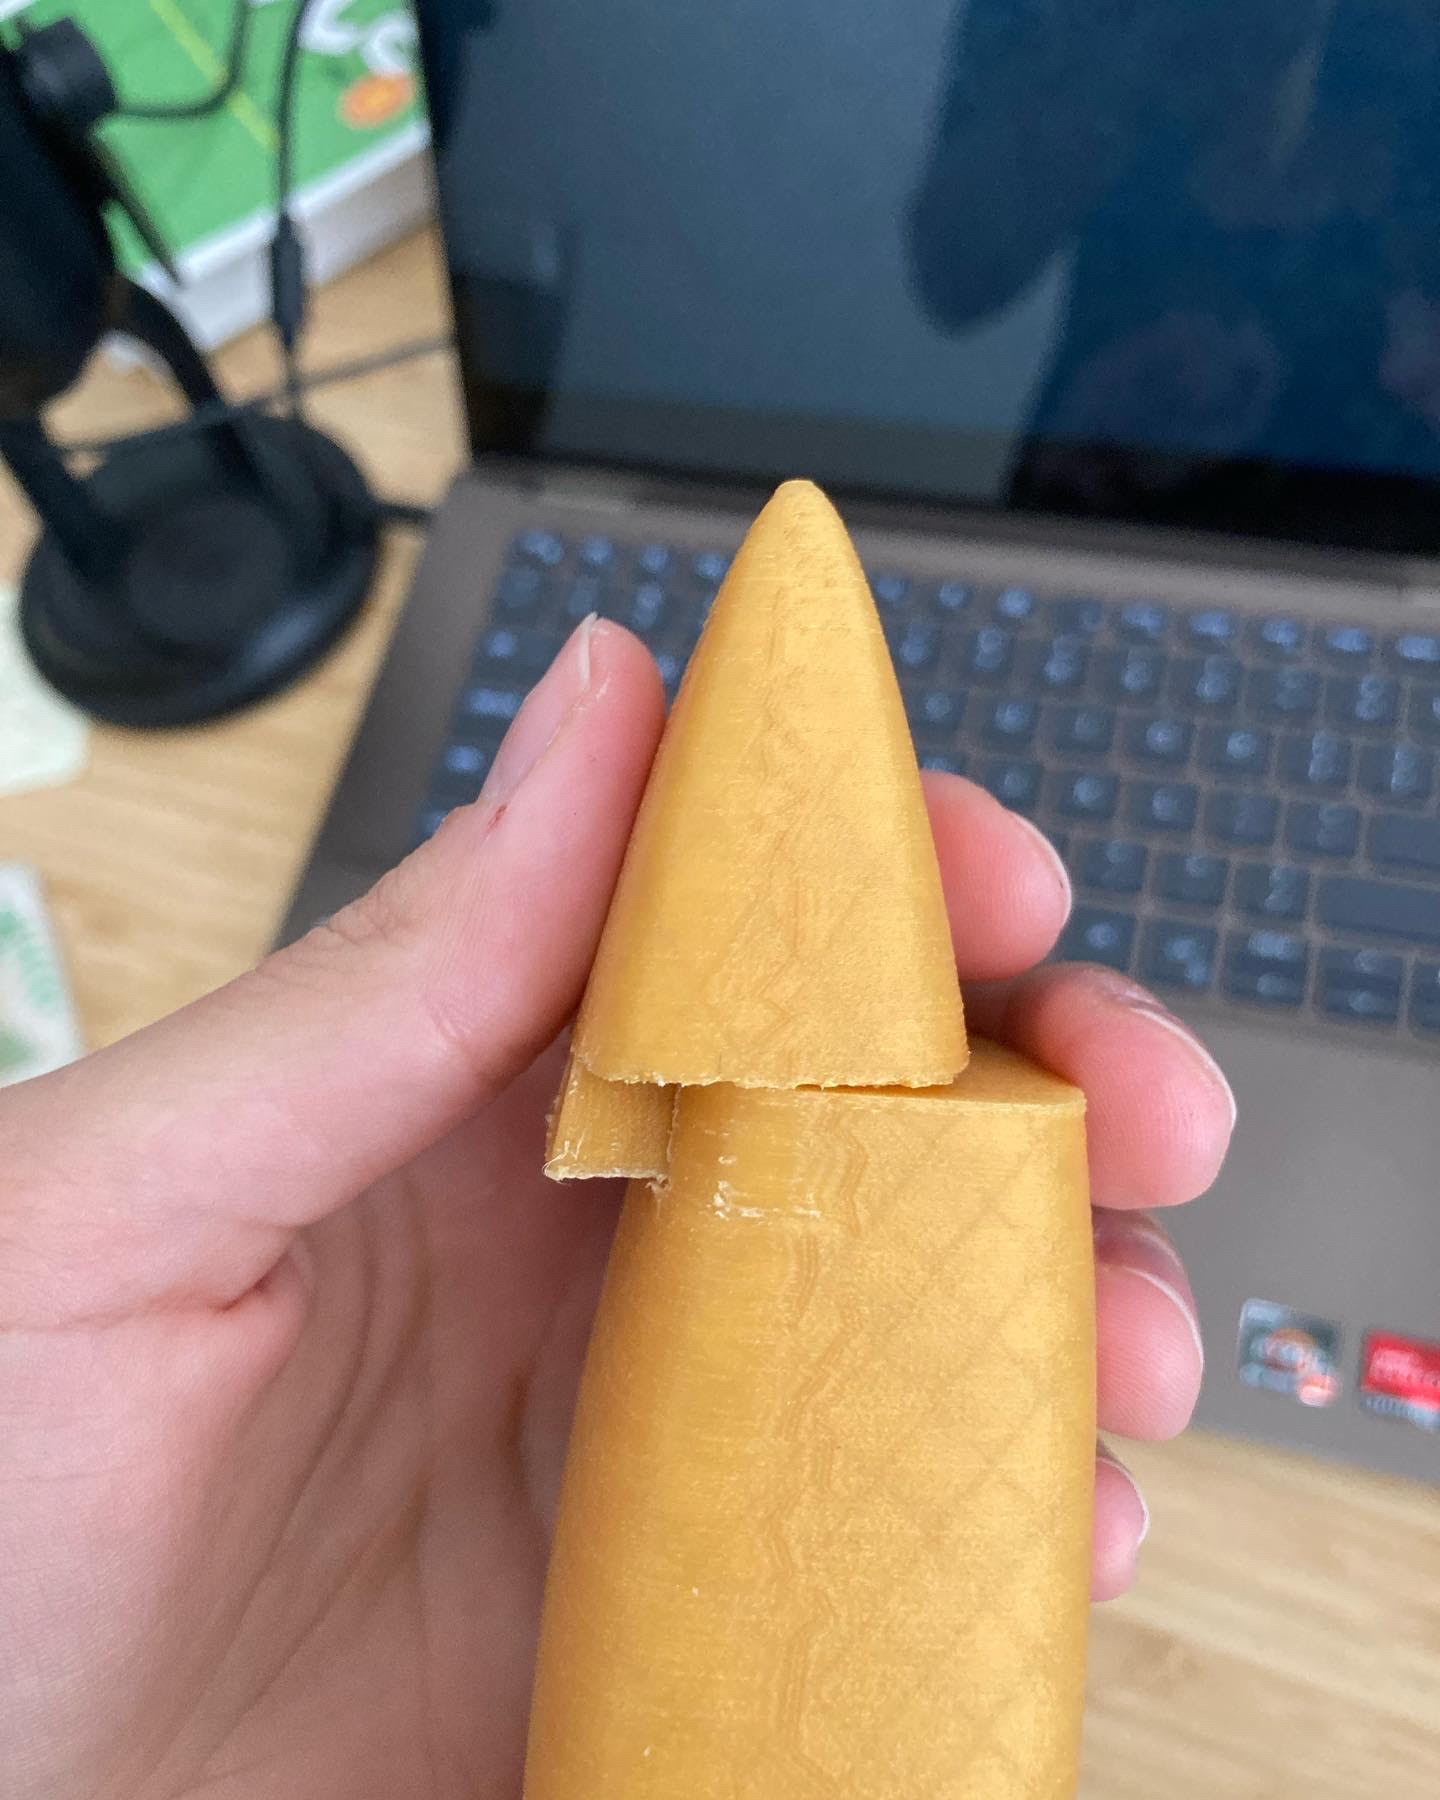
\includegraphics[width=0.5\linewidth]{04_Progress/Figs/clip.jpg}
    \caption{3D Printed Model: Testing front attachment clip stability}
    \label{fig:3Dmodel}
\end{figure}

\section{Experimental Setup}
\label{sec:Experimental Setup}
The main experimental setup so far has largely been conducted through various software. Python was used to edit the aircraft generation code provided by Professor Dries Verstraete provided, in order to develop a MAV that is appropriate as a baseline model for further analysis. This model also has to be manufacturable, and hence VSP and FreeCad have also been used in order to produce a reasonable airfoil wing design and to model the overall aircraft for printing. Software such as Cura and PrusaSlicer have also been used in order to 3D print models of current developments. 


\section{Constraints and Assumptions}
\label{sec: Constraints and assumptions}
Major constraints in the development of the model are given below: 

\begin{itemize}
    \item Model must fit within the 4x3 low-speed wind tunnel at The University of Sydney.
    \item Additional space must also be accounted for in the wind tunnel in order to mitigate the wall effect which occurs when testing within a wind tunnel.
    \item The width of the model sizings must be appropriate to both manufacture in a 3D printer and to assemble.
    \item The final designed model must be able to remain as one piece for testing within the wind tunnel with an operating propeller in both a tractor and pusher configuration.
    \item Space must be allocated for major components to fit inside, including the battery and propeller housing.
\end{itemize}

\section{Future Investigation}
\label{sec: Future Investigation}

Future investigation will look into developing the current baseline model further in order to test the same model in an unpropelled, tractor and pusher configuration. An interchangeable empennage and fuselage will be used to change the model from a tractor to pusher configuration and allows for testing of the same baseline in both configurations. Further investigation will involve an experimental investigation of the propeller-wing interaction by analysing the model in a low-speed wind tunnel. Wind tunnel tests are expected to occur from 5$ms^{-1}$ to 25$ms^{-1}$. This is for a range of incident angles which vary from -15$^\circ$ to 15 $^\circ$. The force readings of this data will be gathered using either a \textit{nano17} or a \textit{nano25} force meter. A further data analysis will also be conducted using Python in order to determine the stability, aerodynamic coefficients and influence of the propeller effects on the developed baseline model. 

